\documentclass[11pt,a4paper]{article}
\usepackage[utf8]{inputenc}
\usepackage[T1]{fontenc}
\usepackage{lmodern}
\usepackage[spanish,es-nodecimaldot,es-noshorthands]{babel}
\usepackage{amsmath,amssymb,mathtools}
\usepackage{geometry}
\geometry{a4paper, margin=1.8cm, top=1.8cm, bottom=1.8cm}
\usepackage{booktabs}
\usepackage{array}
\usepackage{graphicx}
\usepackage{float}
\usepackage{tikz}
\usetikzlibrary{babel,arrows.meta,decorations.pathmorphing,calc}
\usepackage{hyperref}
\hypersetup{colorlinks=true, linkcolor=blue!80!black, urlcolor=blue!80!black, citecolor=blue!80!black}

\title{\textbf{Resolución del Ejercicio 1: Mecánica Lagrangiana y Dinámica}\\[0.2em]
\large Convocatoria de Enero (Curso 2025--2026) --- Mecánica y Ondas I (UCO)}
\author{\textbf{Marcus}}
\date{}

\begin{document}
\maketitle
\vspace{-1.5em}

% ==============================================================================
% APARTADO B
% ==============================================================================
\section*{Apartado b) Grados de Libertad, Coordenadas y Lagrangiana}

\begin{figure}[H]
\centering
\begin{tikzpicture}[scale=0.92, >=Stealth]
    % Ejes coordenados
    \draw[-{Latex[length=3mm, width=2mm]}, thick, gray!80] (-3.0, 0) -- (3.4, 0) node[right, black] {$x$};
    \draw[-{Latex[length=3mm, width=2mm]}, thick, gray!80] (0, -3.5) -- (0, 3.0) node[above, black] {$y$};
    \node[below left] at (0,0) {$O$};
    
    % Aro vertical de radio R
    \draw[line width=1.5pt, color=blue!75!black] (0,0) circle (1.9cm);
    \node[above left, blue!75!black] at (-1.3, 1.3) {Aro (radio $R$)};
    
    % Gravedad con punta rellena y bien definida
    \draw[-{Latex[length=4mm, width=2.5mm]}, line width=1.4pt, red!80!black] (2.7, 2.1) -- (2.7, 0.9) node[midway, right=2pt] {$\vec{g} = -g\hat{\jmath}$};

    % Ángulo theta desde la vertical descendente (-y)
    \def\ang{38} % ángulo en grados
    \coordinate (O) at (0,0);
    \coordinate (A) at ({1.9*sin(\ang)}, {-1.9*cos(\ang)});
    \coordinate (M) at ({3.6*sin(\ang)}, {-3.6*cos(\ang)});
    
    % Línea vertical descendente (referencia para theta)
    \draw[dashed, thick, gray!70] (0,0) -- (0,-3.2);
    
    % Radio R desde O hasta A
    \draw[thick, blue!80!black] (O) -- (A) node[midway, left=2pt] {$R$};
    
    % Arco y etiqueta del ángulo theta
    \draw[-{Latex[length=2.5mm, width=1.8mm]}, thick, orange!90!black] (0,-1.1) arc (-90:{-90+\ang}:1.1);
    \node[orange!90!black] at (0.35, -1.4) {$\theta$};

    % Punto de enganche A sobre el aro
    \filldraw[fill=orange!90, draw=black, thick] (A) circle (2.8pt);
    \node[above left=1pt, black] at (A) {$A$};

    % Resorte desde A hasta la masa m
    \draw[decoration={aspect=0.35, segment length=2.2mm, amplitude=2.4mm, coil}, decorate, thick, green!50!black] (A) -- (M);
    \node[right=6pt, green!40!black] at ($ (A)!0.5!(M) $) {$r(t)$};

    % Masa puntual m
    \filldraw[fill=red!80!black, draw=black, thick] (M) circle (4.2pt);
    \node[below right=2pt, black] at (M) {$m$};

    % Proyecciones cartesianas de la masa m
    \draw[dotted, thick, gray!60] (M) -- ({3.6*sin(\ang)}, 0) node[above, black, font=\footnotesize] {$x_m$};
    \draw[dotted, thick, gray!60] (M) -- (0, {-3.6*cos(\ang)}) node[left, black, font=\footnotesize] {$y_m$};
\end{tikzpicture}
\vspace{-0.5em}
\caption{Representación esquemática del sistema: el punto de enganche $A$ desliza sin fricción sobre el aro vertical de radio $R$, manteniendo el resorte de longitud $r(t)$ alineado radialmente con la masa puntual $m$ bajo la acción del peso $\vec{P} = -mg\hat{\jmath}$.}
\label{fig:diagrama_aro_resorte}
\end{figure}

\textbf{1. Determinación de los grados de libertad:}\\
El sistema está constituido por un aro vertical rígido de radio $R$ centrado en el origen $O$, sobre el cual desliza sin rozamiento el punto de enganche $A$ de un resorte de longitud natural $l_0$, constante $k$ y masa despreciable. Del otro extremo pende una masa puntual $m$ bajo la acción de la gravedad (Figura~\ref{fig:diagrama_aro_resorte}).
\begin{itemize}
    \item Como el enganche y el resorte no tienen masa ($m_A = 0$), el equilibrio de fuerzas sobre el extremo $A$ exige que $\sum \vec{F}_A = \vec{N}_{\text{aro}} + \vec{F}_{\text{resorte}} = \vec{0}$.
    \item Al ser el aro liso, la fuerza de reacción vincular $\vec{N}_{\text{aro}}$ no tiene componente tangencial y es puramente radial. Por tanto, la fuerza del resorte debe ser también radial, lo que obliga al resorte a mantenerse alineado en todo instante con la recta que une el centro $O$ con el punto $A$.
\end{itemize}
El movimiento de la masa $m$ en el plano vertical queda completamente descrito por dos variables independientes, por lo que el sistema tiene \textbf{2 grados de libertad} ($l = 2$).

\textbf{2. Elección de coordenadas generalizadas:}\\
Se eligen como coordenadas generalizadas $q = (r, \theta)$:
\begin{itemize}
    \item $\theta \in [-\pi, \pi]$: ángulo de la dirección radial respecto a la vertical descendente (semieje $-y$).
    \item $r > 0$: longitud instantánea del resorte (de modo que la elongación es $\Delta l = r - l_0$).
\end{itemize}
La distancia de la masa $m$ al centro del aro $O$ es $\rho = R + r$. Su vector de posición en coordenadas cartesianas es:
\begin{equation}
\vec{r}_m = (R + r)\sin\theta\,\hat{\imath} - (R + r)\cos\theta\,\hat{\jmath}.
\end{equation}
Derivando respecto al tiempo, la velocidad y su módulo al cuadrado resultan:
\begin{equation}
\vec{v}_m = \dot{r}\,\hat{u}_r + (R + r)\dot{\theta}\,\hat{u}_\theta \implies v_m^2 = \dot{r}^2 + (R + r)^2\dot{\theta}^2.
\end{equation}

\textbf{3. Obtención de la función Lagrangiana:}\\
Al ser despreciable la masa del resorte, la energía cinética total $T$ corresponde exclusivamente a la partícula $m$:
\begin{equation}
T = \frac{1}{2}m v_m^2 = \frac{1}{2}m\left[ \dot{r}^2 + (R + r)^2\dot{\theta}^2 \right].
\end{equation}
Tomando como origen de energía potencial gravitatoria el centro $O$ ($y = 0$), la energía potencial total $U = U_e + U_g$ es:
\begin{equation}
U(r, \theta) = \frac{1}{2}k(r - l_0)^2 + mgy = \frac{1}{2}k(r - l_0)^2 - mg(R + r)\cos\theta.
\end{equation}
La función Lagrangiana del sistema $L = T - U$ queda determinada por:
\begin{equation}
\boxed{L(r, \theta, \dot{r}, \dot{\theta}) = \frac{1}{2}m\left[ \dot{r}^2 + (R + r)^2\dot{\theta}^2 \right] - \frac{1}{2}k(r - l_0)^2 + mg(R + r)\cos\theta.}
\end{equation}

% ==============================================================================
% APARTADO C
% ==============================================================================
\section*{Apartado c) Ecuaciones del Movimiento y Constante del Movimiento}

\textbf{1. Ecuaciones de Euler-Lagrange:}\\
Aplicando las ecuaciones de Euler-Lagrange $\frac{d}{dt}\left(\frac{\partial L}{\partial \dot{q}_i}\right) - \frac{\partial L}{\partial q_i} = 0$:
\begin{itemize}
    \item Para la coordenada radial $r(t)$:
    \begin{align*}
    \frac{\partial L}{\partial \dot{r}} = m\dot{r}, \qquad \frac{d}{dt}\left(\frac{\partial L}{\partial \dot{r}}\right) = m\ddot{r}, \qquad \frac{\partial L}{\partial r} = m(R + r)\dot{\theta}^2 - k(r - l_0) + mg\cos\theta.
    \end{align*}
    \begin{equation}
    \boxed{\ddot{r} = (R + r)\dot{\theta}^2 - \frac{k}{m}(r - l_0) + g\cos\theta.} \label{eq:el_r}
    \end{equation}
    
    \item Para la coordenada angular $\theta(t)$:
    \begin{align*}
    \frac{\partial L}{\partial \dot{\theta}} = m(R + r)^2\dot{\theta}, \qquad \frac{d}{dt}\left(\frac{\partial L}{\partial \dot{\theta}}\right) = m(R + r)^2\ddot{\theta} + 2m(R + r)\dot{r}\dot{\theta}, \qquad \frac{\partial L}{\partial \theta} = -mg(R + r)\sin\theta.
    \end{align*}
    Dividiendo entre $m(R + r) \neq 0$:
    \begin{equation}
    \boxed{(R + r)\ddot{\theta} + 2\dot{r}\dot{\theta} + g\sin\theta = 0 \iff \ddot{\theta} = -\frac{2\dot{r}\dot{\theta} + g\sin\theta}{R + r}.} \label{eq:el_th}
    \end{equation}
\end{itemize}

\textbf{2. Determinación de la constante del movimiento:}\\
Dado que las ligaduras no dependen explícitamente del tiempo (sistema esclerónomo) y la Lagrangiana tampoco contiene el tiempo de forma explícita ($\partial L/\partial t = 0$), la integral de energía de Jacobi se conserva:
\begin{equation}
\tilde{H} = \dot{r}\frac{\partial L}{\partial \dot{r}} + \dot{\theta}\frac{\partial L}{\partial \dot{\theta}} - L = 2T - (T - U) = T + U \equiv E = \text{constante}.
\end{equation}
Por tanto, la constante del movimiento es la \textbf{energía mecánica total}:
\begin{equation}
\boxed{E = \frac{1}{2}m\left[ \dot{r}^2 + (R + r)^2\dot{\theta}^2 \right] + \frac{1}{2}k(r - l_0)^2 - mg(R + r)\cos\theta.}
\end{equation}
Podemos comprobarlo directamente calculando su derivada temporal total y sustituyendo las ecuaciones del movimiento:
\begin{align*}
\frac{dE}{dt} &= \dot{r}\left[m\ddot{r} - m(R+r)\dot{\theta}^2 + k(r-l_0) - mg\cos\theta\right] \\
&\quad + \dot{\theta}\left[m(R+r)^2\ddot{\theta} + 2m(R+r)\dot{r}\dot{\theta} + mg(R+r)\sin\theta\right] = 0.
\end{align*}

% ==============================================================================
% APARTADO D
% ==============================================================================
\section*{Apartado d) Lagrangiana Auxiliar y Fuerza de Ligadura sobre el Aro}

Para calcular la fuerza de ligadura normal que el aro ejerce sobre el resorte, tratamos la posición radial del punto de enganche como una coordenada libre $\rho_A(t)$. La masa $m$ se sitúa entonces en $\vec{r}_m = (\rho_A + r)\hat{u}_r$, con velocidad al cuadrado:
\begin{equation}
v_m^2 = (\dot{\rho}_A + \dot{r})^2 + (\rho_A + r)^2\dot{\theta}^2.
\end{equation}
La Lagrangiana del sistema no restringido resulta:
\begin{equation}
L_0 = \frac{1}{2}m\left[ (\dot{\rho}_A + \dot{r})^2 + (\rho_A + r)^2\dot{\theta}^2 \right] - \frac{1}{2}k(r - l_0)^2 + mg(\rho_A + r)\cos\theta.
\end{equation}
La condición de apoyo sobre el aro impone la ligadura $f(\rho_A) = \rho_A - R = 0$. Introduciendo el multiplicador de Lagrange $\lambda(t)$, planteamos la \textbf{Lagrangiana auxiliar}:
\begin{equation}
\boxed{L^*(\rho_A, r, \theta, \dot{\rho}_A, \dot{r}, \dot{\theta}, \lambda) = L_0 + \lambda(\rho_A - R).}
\end{equation}
Las ecuaciones de Euler-Lagrange asociadas a $L^*$ son:
\begin{enumerate}
    \item Para $\lambda$: $\frac{\partial L^*}{\partial \lambda} = 0 \implies \rho_A(t) = R \implies \dot{\rho}_A = 0, \quad \ddot{\rho}_A = 0$.
    \item Para la coordenada $\rho_A$:
    \begin{equation*}
    \frac{d}{dt}\left(\frac{\partial L^*}{\partial \dot{\rho}_A}\right) - \frac{\partial L^*}{\partial \rho_A} = 0 \implies m(\ddot{\rho}_A + \ddot{r}) - \left[ m(\rho_A + r)\dot{\theta}^2 + mg\cos\theta + \lambda \right] = 0.
    \end{equation*}
    Sustituyendo $\rho_A = R$ y $\ddot{\rho}_A = 0$:
    \begin{equation}
    \lambda = m\ddot{r} - m(R + r)\dot{\theta}^2 - mg\cos\theta. \label{eq:lambda_exp}
    \end{equation}
    \item Para la coordenada radial $r$:
    \begin{equation*}
    \frac{d}{dt}\left(\frac{\partial L^*}{\partial \dot{r}}\right) - \frac{\partial L^*}{\partial r} = 0 \implies m(\ddot{\rho}_A + \ddot{r}) - \left[ m(\rho_A + r)\dot{\theta}^2 - k(r - l_0) + mg\cos\theta \right] = 0.
    \end{equation*}
    Con $\rho_A = R$ y $\ddot{\rho}_A = 0$:
    \begin{equation}
    m\ddot{r} - m(R + r)\dot{\theta}^2 - mg\cos\theta = -k(r - l_0). \label{eq:r_aux_exp}
    \end{equation}
\end{enumerate}
Igualando las expresiones \eqref{eq:lambda_exp} y \eqref{eq:r_aux_exp}, se obtiene el multiplicador de Lagrange:
\begin{equation}
\boxed{\lambda(t) = -k(r(t) - l_0).}
\end{equation}
Al estar la ligadura dada por $f(\rho_A) = \rho_A - R = 0$, la fuerza generalizada es $Q_{\rho_A} = \lambda \frac{\partial f}{\partial \rho_A} = \lambda$. Por tanto, la fuerza normal que el aro ejerce sobre el resorte es:
\begin{equation}
\boxed{\vec{N}_{\text{aro}} = \lambda\,\hat{u}_r = -k(r - l_0)\hat{u}_r.}
\end{equation}
\textbf{Interpretación física:} Esta fuerza equilibra directamente la acción elástica del resorte:
\begin{itemize}
    \item Si el muelle está estirado ($r > l_0$), tira del enganche hacia afuera y el aro reacciona ejerciendo una fuerza hacia el centro ($\vec{N}_{\text{aro}}$ centrípeta, $\lambda < 0$).
    \item Si el muelle está comprimido ($r < l_0$), empuja hacia adentro y el aro reacciona empujando hacia afuera ($\vec{N}_{\text{aro}}$ centrífuga, $\lambda > 0$).
\end{itemize}

% ==============================================================================
% ANÁLISIS DEL MOVIMIENTO Y CASOS LÍMITE
% ==============================================================================
\section*{Análisis del Movimiento y Casos Límite}

\textbf{1. Posición de equilibrio y pequeñas oscilaciones:}\\
Anulando velocidades y aceleraciones en las ecuaciones del movimiento, se obtiene la posición de equilibrio estático en el punto más bajo del aro:
\begin{equation}
\theta_{\text{eq}} = 0, \qquad r_{\text{eq}} = l_0 + \frac{mg}{k}.
\end{equation}
Para desplazamientos pequeños alrededor del equilibrio, $\eta(t) = r(t) - r_{\text{eq}} \ll r_{\text{eq}}$ y $\theta \ll 1$, podemos aproximar $\sin\theta \approx \theta$, $\cos\theta \approx 1$ y despreciar los términos con productos de velocidades. Con ello, las ecuaciones se desacoplan en dos osciladores armónicos:
\begin{equation}
\ddot{\eta} + \omega_r^2 \eta = 0, \qquad \ddot{\theta} + \omega_\theta^2 \theta = 0,
\end{equation}
cuyas frecuencias naturales de oscilación son:
\begin{equation}
\boxed{\omega_r = \sqrt{\frac{k}{m}}, \qquad \omega_\theta = \sqrt{\frac{g}{R + l_0 + \frac{mg}{k}}}.}
\end{equation}
Cuando la amplitud de oscilación es mayor, ambos modos se acoplan. En particular, si los parámetros satisfacen $\omega_r \approx 2\omega_\theta$, se observa una transferencia resonante de energía entre el modo radial y el angular.

\textbf{2. Casos límite:}\\
A partir de las ecuaciones generales podemos comprobar varios comportamientos límite conocidos:
\begin{itemize}\setlength{\itemsep}{1pt}\setlength{\parskip}{0pt}
    \item \textbf{Muelle muy rígido ($k \to \infty$):} La elongación se anula ($r(t) \to l_0$, $\dot{r} \to 0$) y la longitud total pasa a ser fija, $L = R + l_0$. La ecuación angular se reduce a $(R + l_0)\ddot{\theta} + g\sin\theta = 0$, que coincide con la de un péndulo simple.
    \item \textbf{Aro de radio nulo ($R \to 0$):} El punto de suspensión se fija en el origen de coordenadas $O(0,0)$, recuperando el modelo del péndulo elástico plano.
    \item \textbf{Gravedad nula ($g \to 0$):} El ángulo $\theta$ se convierte en una coordenada cíclica ($\partial L/\partial \theta = 0$). Como consecuencia del teorema de Noether, se conserva el momento canónico conjugado $p_\theta = m(R+r)^2\dot{\theta}$, que equivale al momento angular respecto a $O$.
\end{itemize}

\textbf{3. Influencia de los parámetros:}\\
Las expresiones obtenidas permiten anticipar el efecto de cada parámetro físico en la dinámica:
\begin{itemize}\setlength{\itemsep}{1pt}\setlength{\parskip}{0pt}
    \item \textbf{Radio del aro $R$:} Aumenta el brazo inercial del sistema; un radio mayor incrementa el momento de inercia y reduce la frecuencia angular $\omega_\theta$, sin modificar la frecuencia radial $\omega_r$.
    \item \textbf{Constante elástica $k$:} Determina el estiramiento en equilibrio ($\Delta l_{\text{eq}} = mg/k$). Un muelle más blando (menor $k$) permite mayores elongaciones y acopla con más fuerza el término de Coriolis ($2\dot{r}\dot{\theta}$).
    \item \textbf{Masa $m$:} Al aumentar tanto la inercia como el peso, reduce simultáneamente ambas frecuencias de oscilación ($\omega_r \propto m^{-1/2}$ y $\omega_\theta \propto m^{-1/2}$).
\end{itemize}

\textbf{4. Necesidad de la integración numérica:}\\
Las ecuaciones diferenciales \eqref{eq:el_r} y \eqref{eq:el_th} forman un sistema no lineal y acoplado: la aceleración angular depende de la velocidad radial a través del término de Coriolis ($-2\dot{r}\dot{\theta}/(R+r)$), mientras que la aceleración radial incluye el término centrífugo ($(R+r)\dot{\theta}^2$) y la no linealidad gravitatoria. Al no existir una solución analítica en términos de funciones elementales, es necesario resolver las ecuaciones numéricamente para estudiar la evolución temporal del sistema. Durante este proceso, comprobar que la energía mecánica total se mantiene constante sirve como control para confirmar que el método numérico resuelve el movimiento de forma adecuada.

% ==============================================================================
% RESULTADOS DE LA SIMULACIÓN
% ==============================================================================
\newpage
\section*{Resultados de la Simulación Numérica}

Para estudiar el comportamiento dinámico se han integrado numéricamente las ecuaciones del movimiento tomando como condiciones de referencia: $m = 1\,\text{kg}$, $k = 50\,\text{N/m}$, $R = 1\,\text{m}$, $l_0 = 0.5\,\text{m}$ y un ángulo inicial $\theta_0 = 60^\circ$. A continuación se analizan los resultados obtenidos, organizados en dos figuras que recogen la trayectoria espacial, el balance de energía y la verificación de los casos límite.

\subsection*{Dinámica del Sistema y Balance de Energía}
La Figura~\ref{fig:lamina1} ilustra la evolución espacial y temporal de las coordenadas del sistema, así como la conservación de la energía mecánica:

\begin{figure}[H]
\centering
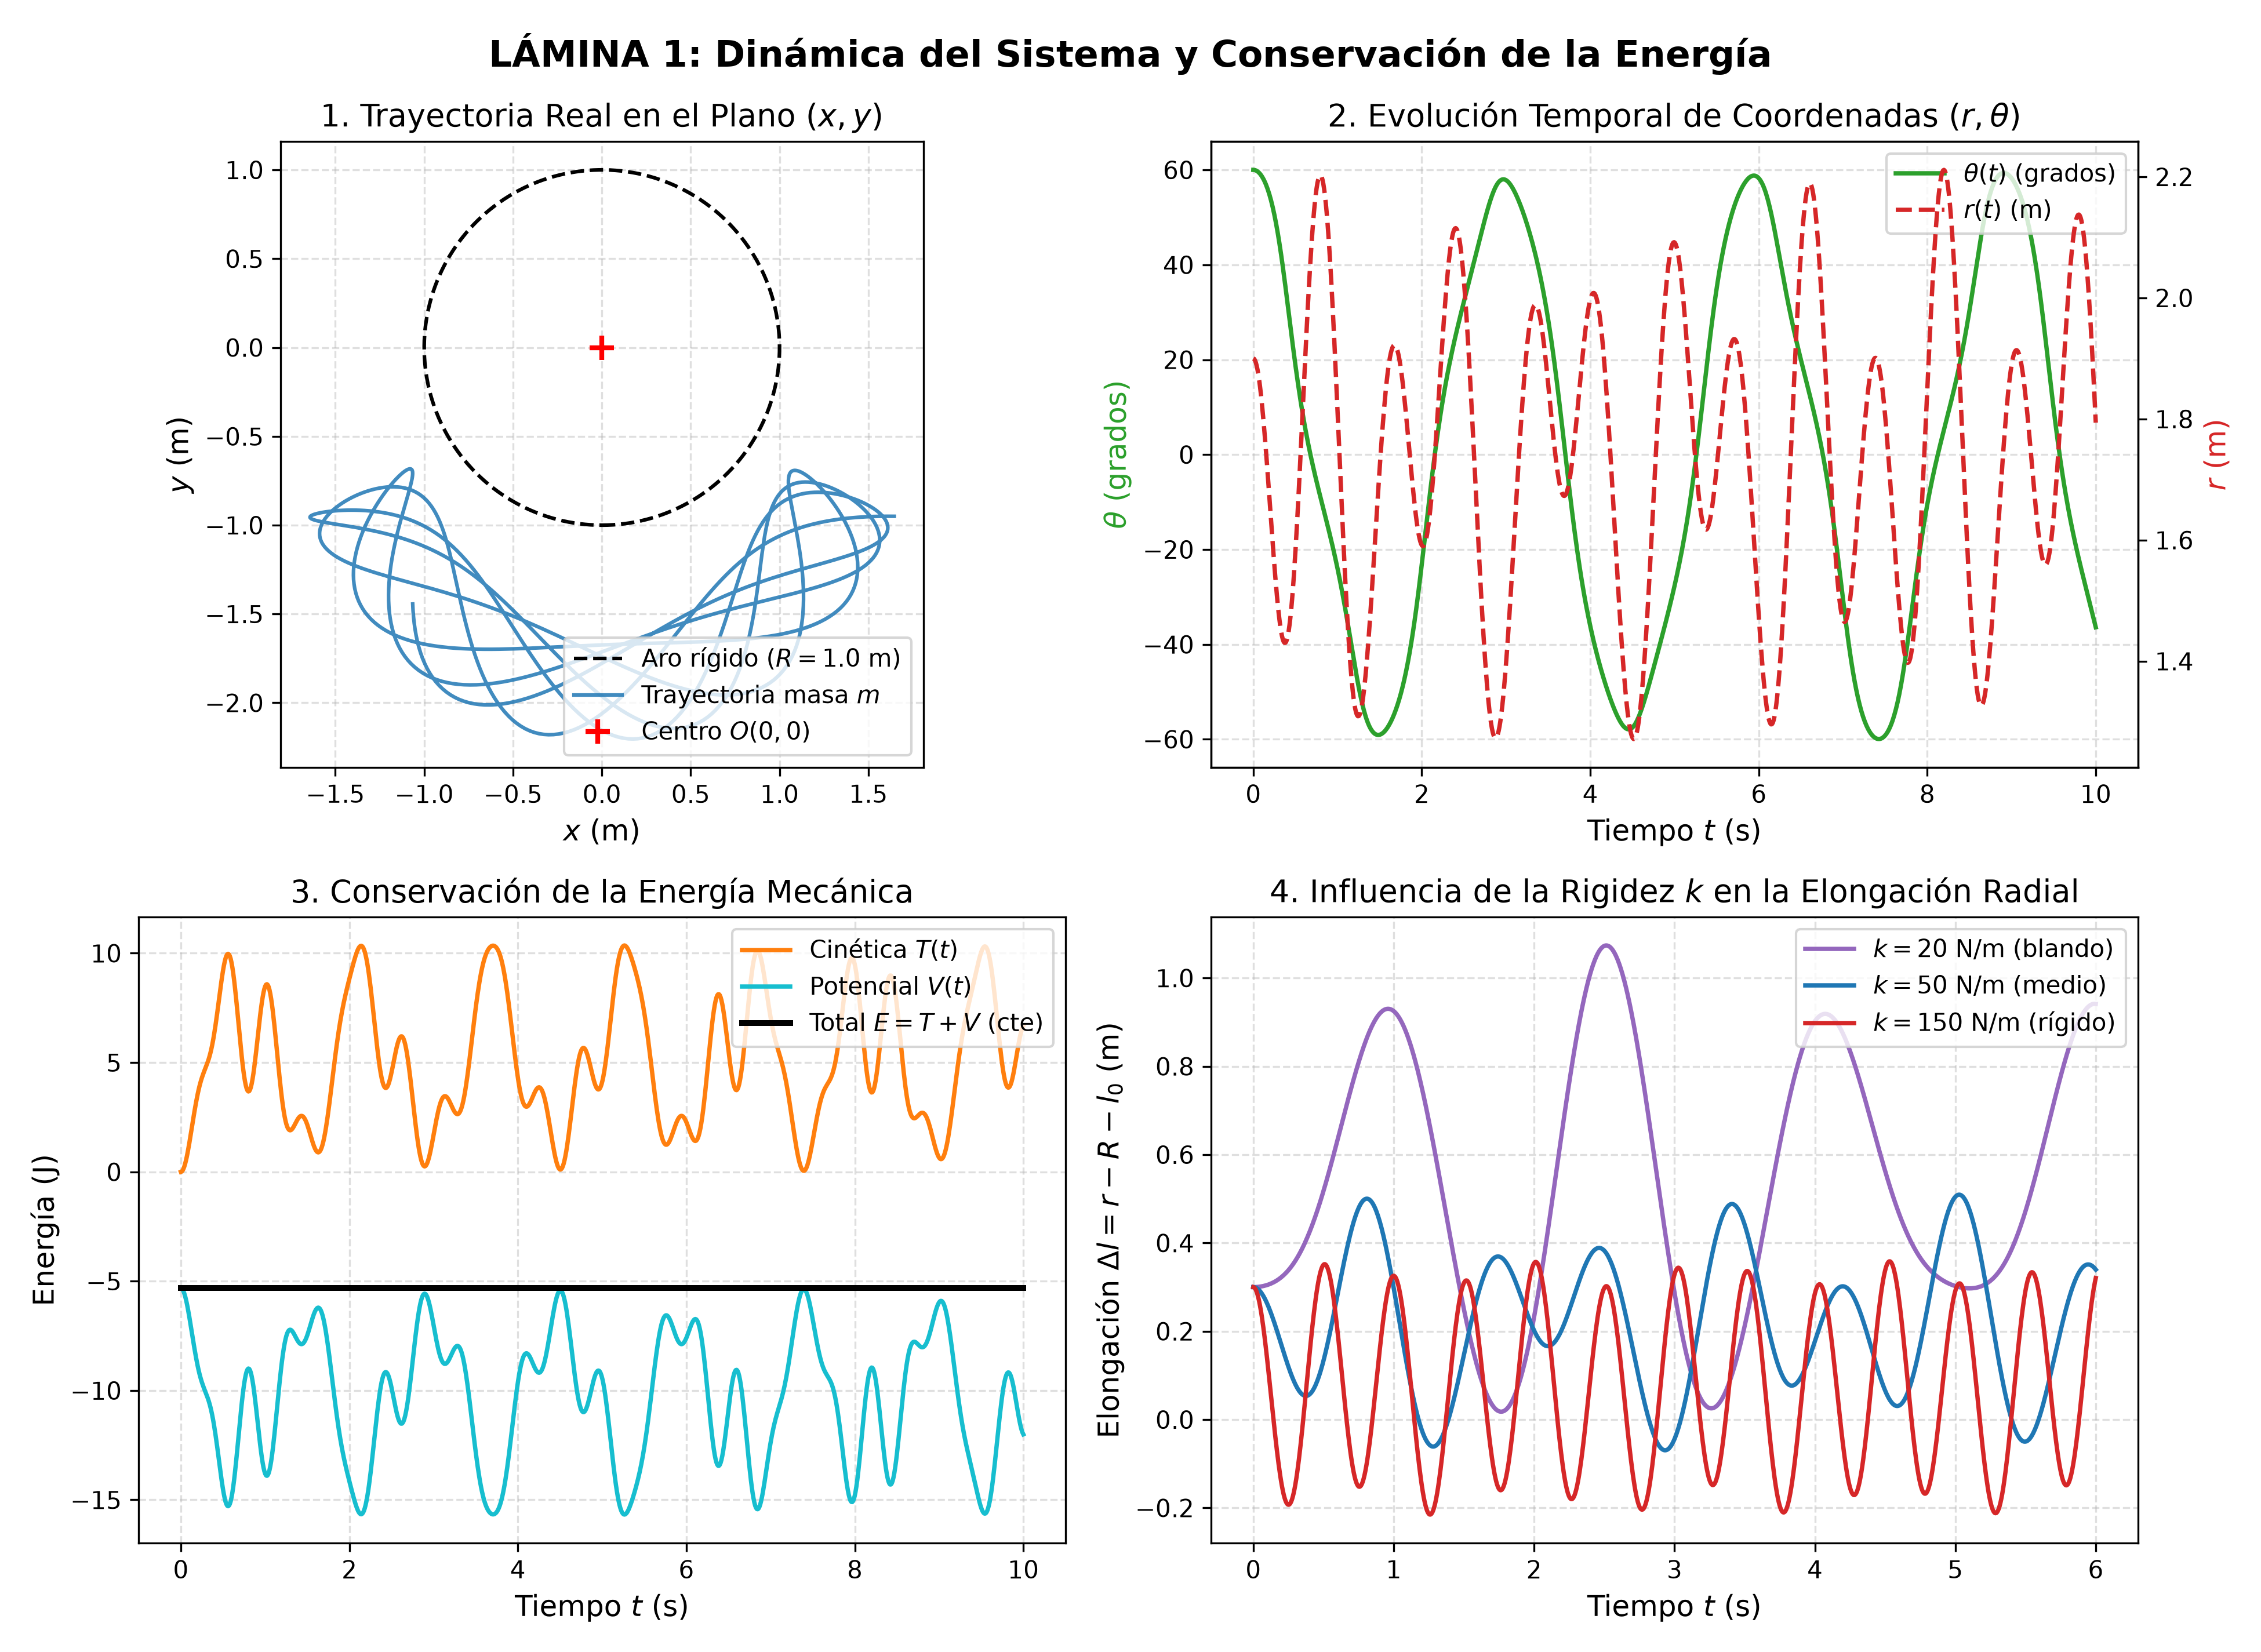
\includegraphics[width=0.76\textwidth]{dossier_lamina_1.png}
\vspace{-0.6em}
\caption{Dinámica temporal y balance energético. (1) Trayectoria en el plano cartesiano de la partícula respecto al aro. (2) Evolución temporal de las coordenadas $(r, \theta)$. (3) Balance de energía cinética, potencial y total. (4) Elongación radial $\Delta l(t)$ para distintos valores de rigidez $k$.}
\label{fig:lamina1}
\end{figure}
\vspace{-0.5em}

\begin{itemize}\setlength{\itemsep}{1pt}\setlength{\parskip}{0pt}
    \item \textbf{Trayectoria en el plano (Panel 1):} La partícula describe un movimiento oscilatorio por debajo del aro. Se aprecia que la trayectoria no es un arco circular cerrado, sino que barre una región bidimensional debido a la combinación del vaivén angular con el estiramiento continuo del muelle.
    \item \textbf{Evolución temporal de $r(t)$ y $\theta(t)$ (Panel 2):} Se observa la coexistencia de dos ritmos de oscilación: una vibración elástica rápida en la coordenada radial $r(t)$ y una oscilación pendular más lenta en el ángulo $\theta(t)$, mostrando el acoplamiento entre ambos grados de libertad.
    \item \textbf{Conservación de la energía (Panel 3):} A lo largo del movimiento se produce un intercambio continuo entre energía cinética $T(t)$ y energía potencial $V(t)$. La energía mecánica total $E = T + V$ se mantiene horizontal y constante a lo largo de toda la integración, lo que indica que el método numérico resuelve el sistema sin introducir pérdidas ni ganancias artificiales de energía.
    \item \textbf{Influencia de la rigidez $k$ (Panel 4):} Al comparar tres valores de rigidez ($k = 20$, $50$ y $150\,\text{N/m}$), se comprueba que un muelle más rígido reduce notablemente la amplitud de estiramiento e incrementa la frecuencia de oscilación, de acuerdo con $\omega_r \approx \sqrt{k/m}$.
\end{itemize}

\newpage
\subsection*{Comprobación de Casos Límite y Fuerza de Ligadura}
La Figura~\ref{fig:lamina2} compara los resultados de la simulación con los comportamientos teóricos deducidos analíticamente:

\begin{figure}[H]
\centering
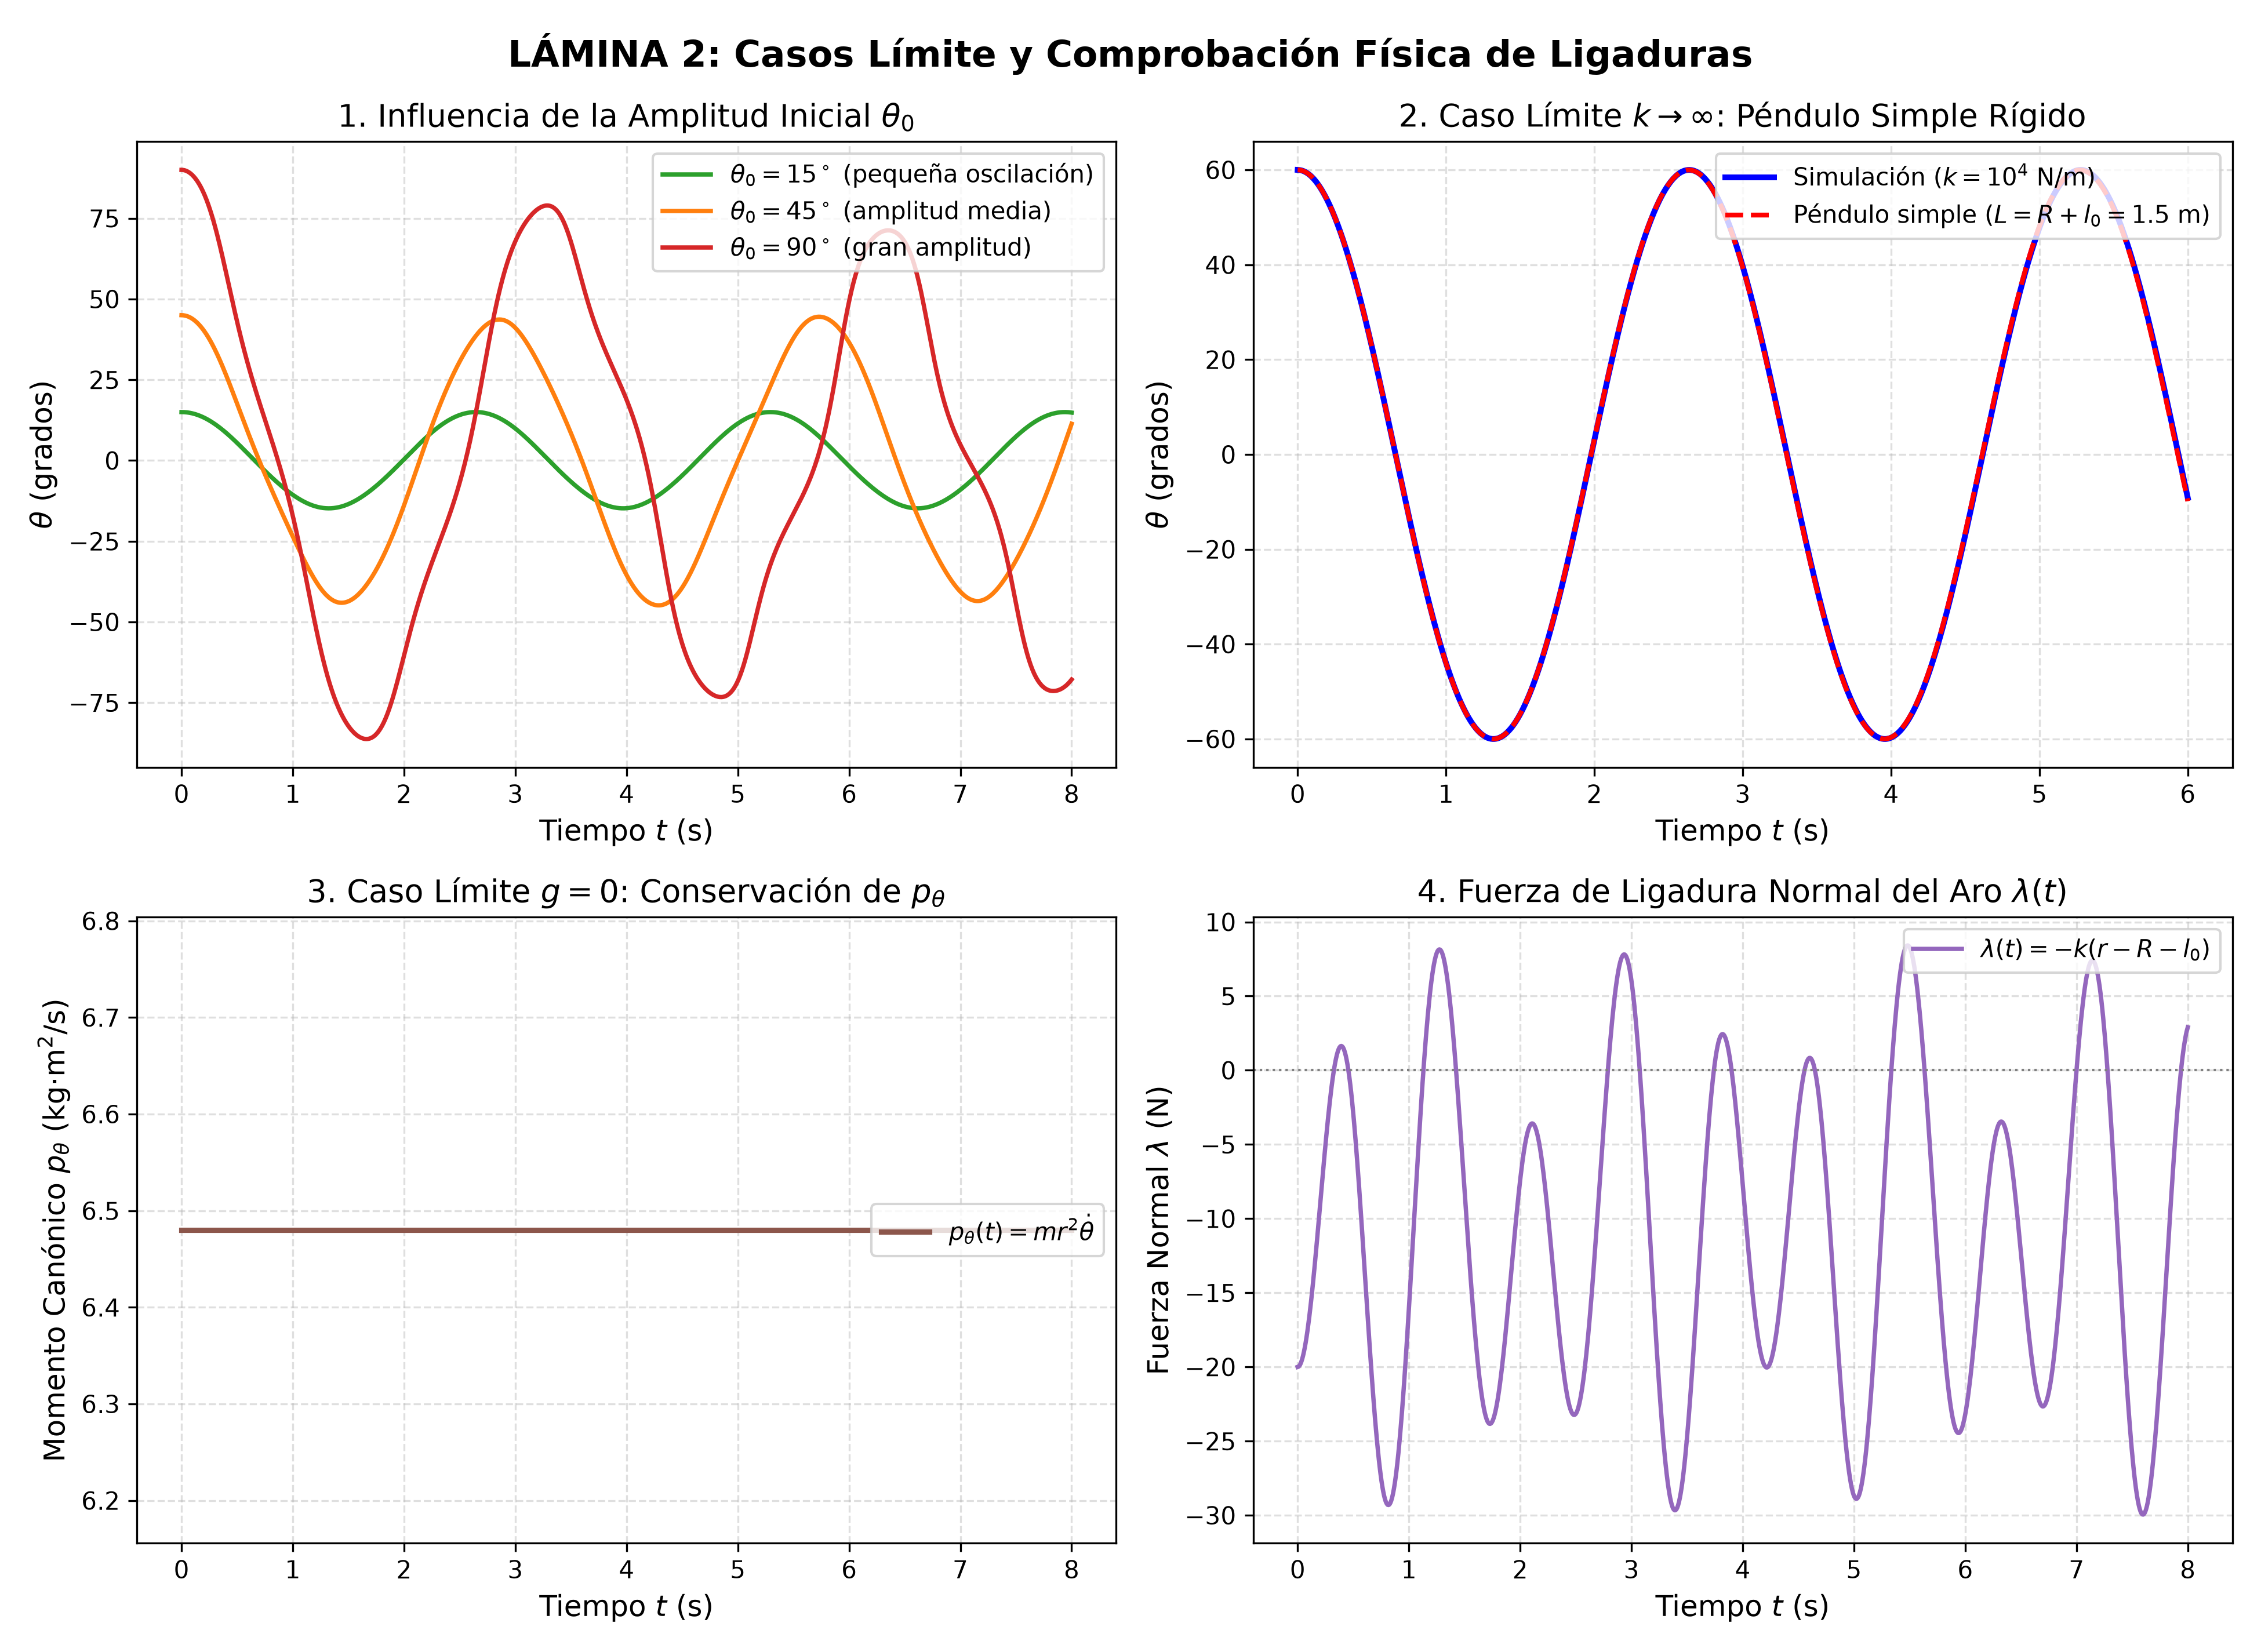
\includegraphics[width=0.61\textwidth]{dossier_lamina_2.png}
\vspace{-0.7em}
\caption{Verificación de límites teóricos y fuerza normal. (1) Influencia de la amplitud inicial $\theta_0$. (2) Caso límite de muelle rígido ($k = 10^4\,\text{N/m}$) comparado con el péndulo simple. (3) Caso de gravedad nula ($g = 0$) y momento canónico $p_\theta$. (4) Fuerza normal de ligadura $\lambda(t)$ ejercida por el aro.}
\label{fig:lamina2}
\end{figure}
\vspace{-0.6em}

\begin{itemize}\setlength{\itemsep}{0pt}\setlength{\parskip}{0pt}
    \item \textbf{Efecto de la amplitud inicial (Panel 1):} Para amplitudes pequeñas ($\theta_0 = 15^\circ$) la oscilación es prácticamente armónica. Para amplitudes grandes ($\theta_0 = 90^\circ$), el término $\sin\theta$ alarga notablemente el período respecto al régimen lineal.
    \item \textbf{Límite de muelle rígido (Panel 2):} Con rigidez muy alta ($k = 10^4\,\text{N/m}$), el resorte apenas se deforma y $\theta(t)$ coincide con la solución de un péndulo simple de longitud $L = R + l_0 = 1.5\,\text{m}$, confirmando la coherencia del modelo con el límite rígido.
    \item \textbf{Límite sin gravedad (Panel 3):} Con $g = 0$, la coordenada $\theta$ es cíclica. La simulación muestra que el momento canónico conjugado $p_\theta = m(R+r)^2\dot{\theta}$ permanece constante en el tiempo, tal como predice el teorema de Noether.
    \item \textbf{Fuerza normal de ligadura (Panel 4):} La fuerza $\lambda(t) = -k(r - l_0)$ que el aro ejerce sobre el enganche oscila en torno a cero: es negativa (hacia el centro) cuando el muelle está estirado ($r > l_0$) y positiva (hacia afuera) cuando está comprimido ($r < l_0$).
\end{itemize}

% ==============================================================================
% CONCLUSIONES
% ==============================================================================
\section*{Conclusiones}
\vspace{-0.2em}
Los resultados principales obtenidos en este trabajo son:
\begin{enumerate}\setlength{\itemsep}{0pt}\setlength{\parskip}{0pt}
    \item El formalismo lagrangiano permite describir el sistema de dos grados de libertad mediante las coordenadas $(r, \theta)$, obteniendo las ecuaciones del movimiento sin necesidad de calcular previamente las fuerzas de ligadura internas.
    \item Las ecuaciones diferenciales resultan acopladas y no lineales por la presencia de aceleraciones de inercia (centrífuga y de Coriolis) y del peso, lo que impide una solución analítica cerrada y justifica la integración numérica.
    \item La simulación numérica confirma los comportamientos teóricos: la energía mecánica total se mantiene constante en el tiempo y los casos límite (péndulo simple para $k \to \infty$ y conservación del momento angular para $g = 0$) concuerdan con los modelos físicos conocidos.
    \item El método de los multiplicadores de Lagrange permite calcular de forma directa la fuerza de reacción normal ejercida por el aro, $\lambda(t) = -k(r - l_0)$, comprobando que el aro equilibra en todo instante la tensión radial del muelle.
\end{enumerate}

\end{document}
